\chapter{Performance prediction through simulation: the HPL case}
\label{chapter:prediction}

The work presented in this chapter has been published at a conference\cite{cornebize:cluster19} and has been submitted
for publication in a journal. The content of this chapter is therefore a near-verbatim copy of these articles. This work
also directly follows my master thesis\cite{cornebize:master_thesis} whose main contribution is summarized in
section\ref{sec:prediction:emulation} for the sake of completeness.

\section{High Performance Linpack}%
\label{sec:prediction:hpl}

    \subsection{The benchmark}%
    \label{sub:hpl:benchmark}

        \begin{figure}[ht]
            \newcommand{\mykwfn}[1]{{\textbf{\textsf{#1}}}}%
            \SetAlFnt{\textsf}%
            \SetKwSty{mykwfn}%
            \SetKw{KwStep}{step}%
            \centering
            \begin{minipage}[m]{0.5\linewidth}
                % \vspace{0.3cm} % ugly, could not align the drawing with the algorithm with minipages or tabular...
                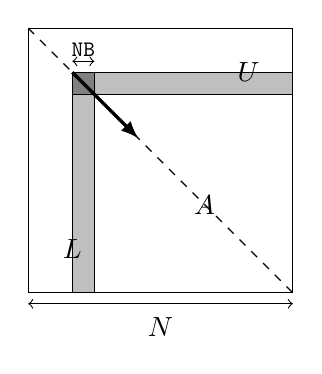
\begin{tikzpicture}[scale=0.28]
                    \draw (0, 0) -- (0, 12) -- (12, 12) -- (12, 0) -- cycle;
                    \foreach \i in {2}{
                        \draw [fill=lightgray] (\i, 0) -- (\i, 12-\i) -- (12, 12-\i) -- (12, 0) -- cycle;
                        \draw [fill=gray] (\i, 12-\i) -- (\i, 12-\i-1) -- (\i+1, 12-\i-1) -- (\i+1, 12-\i) -- cycle;
                        \draw[very thick, -latex] (\i,12-\i) -- (\i+2,12-\i-2);
                        \draw[<->] (\i, 12-\i+0.5) -- (\i+1, 12-\i+0.5) node [pos=0.5, yshift=+0.15cm] {\scalebox{.8}{\texttt{NB}}};
                    }
                    \foreach \i in {3}{
                        \draw [fill=white] (\i, 0) -- (\i, 12-\i) -- (12, 12-\i) -- (12, 0) -- cycle;
                        \draw (\i,12-\i) -- (\i,0);
                        \draw[very thick, -latex] (\i,12-\i) -- (\i+2,12-\i-2);
                    }
                    \draw[dashed] (0, 12) -- (12, 0);
                    \node(L) at (2, 2) {\ensuremath{\boldsymbol{L}}};
                    \node(U) at (10, 10) {\ensuremath{\boldsymbol{U}}};
                    \node(A) at (8, 4) {\ensuremath{\boldsymbol{A}}};
                    \draw[<->] (0, -0.5) -- (12, -0.5) node [pos=0.5, yshift=-0.3cm] {$N$};
                \end{tikzpicture}
            \end{minipage}%
            \begin{minipage}[m]{0.5\linewidth}
                \begin{algorithm}[H]
                    allocate and initialize $A$\;
                    \For{$k=N$ \KwTo $0$ \KwStep \texttt{NB}}{
                        allocate the panel\;
                        factor the panel\;
                        broadcast the panel\;
                        update the sub-matrix;
                    }
                \end{algorithm}
                \vspace{1em}
            \end{minipage}\vspace{-.5em}
            \caption{Overview of High Performance Linpack}\vspace{-1.5em}
            \label{fig:hpl_overview}
        \end{figure}

        In this work, we use the freely-available reference-implementation of HPL\cite{hpl}, which relies on MPI.  HPL
        implements a matrix factorization based on a right-looking variant of the LU factorization with row partial pivoting
        and allows multiple look-ahead depths. The principle of the factorization is depicted in
        Figure\ref{fig:hpl_overview}. It consists of a series of panel factorizations followed by an update of the trailing
        sub-matrix.  HPL uses a two-dimensional block-cyclic data distribution of $A$ and implements several custom MPI
        collective communication algorithms to efficiently overlap communications with computations.
        The main parameters of HPL are:
        \begin{itemize}
            \item \texttt{N} is the order of the square matrix $A$.
            \item \texttt{NB} is the \emph{blocking factor}, \ie the granularity at which HPL operates when panels are
                distributed or worked on.
            \item \texttt{P} and \texttt{Q} denote the number of process rows and the number of process columns,
                respectively.
            \item \texttt{RFACT} determines the panel factorization algorithm. Possible values are Crout, left- or
                right-looking.
            \item \texttt{SWAP} specifies the swapping algorithm used while pivoting. Two algorithms are available: one
                based on \emph{binary exchange} (along a virtual tree topology) and the other one based on a
                \emph{spread-and-roll} (with a higher number of parallel communications). HPL also provides a panel-size
                threshold triggering a switch from one variant to the other.
            \item \texttt{BCAST} sets the algorithm used to broadcast a panel of columns over the process columns. Legacy
                versions of the MPI standard only supported non-blocking point-to-point communications, which is why HPL
                ships with in total 6 self-implemented variants to overlap the time spent waiting for an incoming panel with
                updates to the trailing matrix: \texttt{ring}, \texttt{ring-modified}, \texttt{2-ring},
                \texttt{2-ring-modified}, \texttt{long}, and \texttt{long-modified}. The \texttt{modified} versions
                guarantee that the process right after the root (\ie the process that will become the root in the next
                iteration) receives data first and does not further participate in the broadcast. This process can thereby
                start working on the panel as soon as possible. The \texttt{ring} and \texttt{2-ring} versions each
                broadcast along the corresponding virtual topologies while the \texttt{long} version is a \emph{spread and
                roll} algorithm where messages are chopped into \texttt{Q} pieces. This generally leads to better bandwidth
                exploitation. The \texttt{ring} and \texttt{2-ring} variants rely on \texttt{MPI\_Iprobe}, meaning they
                return control if no message has been fully received yet, hence facilitating partial overlap of
                communication with computations.  In HPL 2.1 and 2.2, this capability has been deactivated for the
                \texttt{long} and \texttt{long-modified} algorithms. A comment in the source code states that some machines
                apparently get stuck when there are too many ongoing messages.
            \item \texttt{DEPTH} controls how many iterations of the outer loop can overlap with each other.
        \end{itemize}

        The sequential complexity of this factorization is \[\mathrm{flop}(N) = \frac{2}{3}N^3 + 2N^2 + \landauO(N)\] where $N$ is
        the order of the matrix to factorize. The time complexity can be approximated by \[T(N) \approx
        \frac{\left(\frac{2}{3}N^3 + 2N^2\right)}{P\cdot{}Q\cdot{}w} + \Theta((P+Q)\cdot{}N^2)\] where $w$ is the flop rate
        of a single node and the second term corresponds to the communication overhead which is influenced by the network
        capacity and the previously listed parameters (\texttt{RFACT}, \texttt{SWAP}, \texttt{BCAST},
        \texttt{DEPTH}, \ldots) and is very difficult to predict.

    \subsection{Typical runs on a supercomputer}%
    \label{sub:hpl:typical_runs}

        Although the TOP500 reports precise information about the core count,
        the peak performance and the effective performance, it provides almost
        no information on how (software versions, HPL parameters, etc.) this
        performance was achieved. Some colleagues agreed to provide us with
        the HPL configuration they used and the output they submitted for
        ranking (see Table\ref{fig:typical_run}).
        In June 2013, the Stampede supercomputer at TACC was ranked
        6th in the TOP500 by achieving \NSI{5168.1}{\tera\flops}. In November
        2017, the Theta supercomputer at ANL was ranked 18th with a performance of \NSI{5884.6}{\tera\flops}
        but required a 28-hour run on the
        whole machine. Finally, we ran HPL ourselves on a Grid'5000 cluster
        named Dahu whose software stack could be fully controlled.

        \begin{table}[hb]
            \caption{Typical runs of HPL}
            \label{fig:typical_run}
            \scalebox{.9}{\begin{tabular}{l|lll}
                \multicolumn{1}{l|}{} & Stampede@TACC & Theta@ANL & Dahu@G5K\\
                \hline
                \texttt{Rpeak}     & \NSI{8520.1}{\tera\flops} & \NSI{9627.2}{\tera\flops} & \NSI{62.26}{\tera\flops}              \\
                $N$         & \Num{3875000}                & \Num{8360352}                & \Num{500000}            \\
                \texttt{NB}        & \Num{1024}                    & 336                      & 128                \\
                $P\times Q$             & 77$\times$78                  & 32$\times$101                 & 32$\times$32            \\
                \texttt{RFACT}     & Crout                    & Left                     & Right              \\
                \texttt{SWAP}      & Binary-exch.             & Binary-exch.             & Binary-exch.       \\
                \texttt{BCAST}     & Long modified            & 2 Ring modified          & 2 Ring             \\
                \texttt{DEPTH}     & 0                        & 0                        & 1                  \\
                \hline
                \texttt{Rmax}      & \NSI{5168.1}{\tera\flops} & \NSI{5884.6}{\tera\flops} & \NSI{24.55}{\tera\flops}              \\
                Duration   & 2 hours                  & 28 hours                 & 1 hour             \\
                Memory    & \NSI{120}{\tera\byte}     & \NSI{559}{\tera\byte}     & \NSI{2}{\tera\byte} \\
                MPI ranks & 1/node                & 1/node                   & 1/core             \\
            \end{tabular}}
        \end{table}


        The performance typically achieved by supercomputers (\texttt{Rmax}) needs to be compared to the much larger
        peak performance (\texttt{Rpeak}). This difference can be attributed to the node usage, to the MPI library, to
        the network topology that may be unable to deal with the intense communication workload, to load imbalance among
        nodes (\eg due to a defect, system noise, \ldots), to the algorithmic structure of HPL, etc. All these factors
        make it difficult to know precisely what performance to expect without running the application at scale.  It is
        clear that due to the level of complexity of both HPL and the underlying hardware, simple performance models
        (analytic expressions based on $N, P, Q$ and estimations of platform characteristics) may be able to provide
        trends but can by no means accurately predict the performance for each configuration (\eg consider the exact
        effect of HPL's six different broadcast algorithms on network contention). Additionally, these expressions do
        not allow engineers to improve the performance through actively identifying performance bottlenecks.  For
        complex optimizations such as partially non-blocking collective communication algorithms intertwined with
        computations, a very faithful modeling of both the application and the platform is required. One goal of this
        thesis was to simulate systems at the scale of Stampede. Given the scale of this scenario (3,785~steps on
        6,006 nodes in two hours), detailed simulations quickly become intractable without significant effort.



\section{Related work}%
\label{sec:prediction:related_work}

    \subsection{Performance prediction}%
    \label{sub:performance_prediction}

        A first approach for estimating the performance of applications like HPL is statistical modeling of the
        application as a whole\cite{hpl_prediction}.  By running the application several times with small and medium
        problem sizes (of a few iterations of large problem sizes) and using simple linear regressions, it is possible
        to predict its makespan for larger sizes with an error of only a few percents and a relatively low cost.
        Unfortunately, the predictions are limited to the same application configuration and studying the influence of
        the number of rows and columns of the virtual grid or of the broadcast algorithms requires a new model and new
        (costly) runs using the whole target machine.  Furthermore, this approach does not allow to study what-if
        scenarios (\eg to evaluate what would happen if the network bandwidth was increased or if node heterogeneity was
        decreased) that are particularly useful when investigating potential performance improvements.

        Simulation provides the details and flexibility missing to such black-box modeling approach. Performance
        prediction of MPI applications through simulation has been widely studied over the last decades but two
        approaches can be distinguished in the literature: offline and online simulation.

        With the most common approach, \emph{offline simulation}, a trace of the application is first obtained on a real
        platform. This trace comprises sequences of MPI operations and CPU bursts and is given as an input to a
        simulator that implements performance models for the CPUs and the network to derive predictions. Researchers
        interested in finding out how their application reacts to changes to the underlying platform can replay the
        trace on commodity hardware at will with different platform models.
        Most HPC simulators available today, notably BigSim\cite{bigsim_04}, Dimemas\cite{dimemas} and
        CODES\cite{CODES}, rely on this approach.  The main limitation of this approach comes from the trace acquisition
        requirement. Not only is a large machine required but the compressed trace of a few iterations (out of several
        thousands) of HPL typically reaches a few hundred MB, making this approach quickly impractical\cite{suter}.
        Worse, tracing an application provides only information about its behavior at the time of the run: slight
        modifications (\eg to communication patterns) may make the trace inaccurate. The behavior of simple applications
        (\eg \texttt{stencil}) can be extrapolated from small-scale traces\cite{scalaextrap,pmac_lspp13} but this fails
        if the execution is non-deterministic, \eg whenever the application relies on non-blocking communication
        patterns, which is unfortunately the case for HPL.

        The second approach discussed in the literature is \emph{online simulation}.  Here, the application is executed
        (emulated) on top of a simulator that is responsible to determine when each process is run. This approach allows
        researchers to study directly the behavior of MPI applications but only a few recent simulators such as SST
        Macro\cite{sstmacro}, SimGrid/SMPI\cite{simgrid} and the closed-source xSim\cite{xsim} support it. To the best
        of our knowledge, only SST Macro and SimGrid/SMPI are mature enough to faithfully emulate HPL. This work relies
        on SimGrid as its performance models and its emulation capabilities seemed quite solid but the proposed
        developments would a priori also be possible with SST.  Note that the HPL emulation described in
        Section\ref{sec:prediction:emulation} should not be confused with the application
        skeletonization\cite{sst_skeleton} commonly used with SST. Skeletons are code extractions of the most important
        parts of a complex application whereas we only modify a few dozens of lines of HPL before emulating it with
        SMPI. Finally, it is important to understand that the proposed approach is intended to help studies at the level
        of the whole machine and application, not the influence of microarchitectural details as intended by
        MUSA\cite{musa_16}.

    \subsection{Simgrid/SMPI}%
    \label{sub:simgrid_smpi}

        SimGrid\cite{simgrid} is a flexible and open-source simulation framework that was originally designed in 2000 to
        study scheduling heuristics tailored to heterogeneous grid computing environments but has later been extended to
        study cloud and HPC infrastructures. The main development goal for SimGrid has been to provide validated performance
        models particularly for scenarios making heavy use of the network.  Such a validation usually consists of comparing
        simulation predictions with results from real experiments to confirm or debunk network and application models.

        SMPI, a simulator based on SimGrid, has been developed and used to simulate unmodified MPI applications written in
        C/C++ or FORTRAN\cite{smpi}.
        The complex network optimizations done in real MPI implementations need to be considered when predicting the
        performance of MPI applications.  For instance, the "eager" and "rendez-vous" protocols are selected based on the
        message size, with each protocol having its own synchronization semantics, which strongly impact performance.  SMPI
        supports different performance modes through a generalization of the LogGPS model.  Another difficult issue is to
        model network topologies and contention. SMPI relies on SimGrid's communication models where each ongoing
        communication is represented as a whole (as opposed to single packets) by a \emph{flow}. Assuming steady-state,
        contention between active communications can then be modeled as a bandwidth sharing problem that accounts for
        non-trivial phenomena (\eg cross-traffic interference\cite{Velho_TOMACS13}). If needed, communications that start or
        end trigger a re-computation of the bandwidth share.  In this fluid model, the time to simulate a message passing
        through the network is independent of its size, which is advantageous for large-scale applications frequently
        sending large messages and orders of magnitude faster than packet-level simulation.  SimGrid does not model
        transient phenomena incurred by the network protocol but accounts for network topology and heterogeneity. Special
        attention to the modeling of collective communication algorithms has also been paid in SMPI, but this is of little
        significance in this article as HPL ships with its own implementation of collective operations.

        SMPI maps every MPI rank of the application onto a lightweight simulation thread. These threads are then run one at
        a time, \ie in mutual exclusion.  Every time a thread enters an MPI call, SMPI takes control and the time that was
        spent computing (isolated from the other threads) since the previous MPI call is injected into the simulator as a
        virtual delay.  This time may be scaled up or down depending on the speed of the simulated machine with respect to
        the simulation machine.
        Recent results report consistent performance predictions within a few percent for standard benchmarks on small-scale
        clusters (up to \(12\times12\) cores \cite{heinrich:hal-01523608} and up to \(128\times1\) cores \cite{smpi}). In
        this thesis, I validate this approach at a much larger scale with HPL, whose emulation comes with at least two
        challenges:
        \begin{itemize}
        \item The time-complexity of the algorithm is \(\Theta(N^3)\) and \(\Theta(N^2)\) communications are performed, with
            \(N\) being very large. The execution on the Stampede cluster took roughly two hours on \Num{6006}~compute
            nodes. Using only a single node, a naive emulation of HPL at the scale of the Stampede run would take about
            500 days if perfect scaling was reached.
        \item The tremendous memory consumption and amount of memory accesses need to be drastically reduced.
        \end{itemize}

\section{Emulating HPL at large scale}%
\label{sec:prediction:emulation}

    In this section, I present the changes to SimGrid and HPL that were required for a scalable simulation.  The
    experiments were done using a single core from nodes of the Nova cluster provided by the Grid'5000
    testbed\cite{grid5000} (\NSI{32}{\giga\byte} of RAM, two 8-core Intel Xeon E5-2620 v4 CPUs, Debian Stretch OS
    (Linux 4.9)).

    \subsection{Speeding Up the Emulation}
        \label{sub:speeding_emulation}

        \subsubsection{Compute Kernel Modeling}
            \begin{figure}[htb]
                \centering
                \subfigure[Non-intrusive macro replacement with a very simple computation model.\label{fig:macro_simple}]{
                    \begin{minipage}[b]{\linewidth}
                        \lstset{frame=bt,language=C,numbers=none,escapechar=|}\lstinputlisting{img/prediction/emulating/HPL_dgemm_macro_simple.c}
                    \end{minipage}}\vspace{-1em}
                \subfigure[Gain in terms of simulation time.\label{fig:kernel_sampling}]{
                    \begin{minipage}[b]{\linewidth}
                        
\includegraphics[width=\linewidth,page=2]{img/prediction/emulating/kernel_modeling.pdf}
                    \end{minipage}}%\vspace{-1em}
                \caption{Replacing the calls to computationally expensive functions by a model allows to emulate HPL at
                a larger scale.}\vspace{-1em}
            \end{figure}

            HPL heavily relies on BLAS kernels such as \texttt{dgemm} (for matrix-matrix multiplication) or \texttt{dtrsm}
            (for solving an  \(A\cdot x=b\) equation). The analysis of an HPL simulation with \(64\) processes and a very
            small matrix of order \Num{30000} showed that about \(\NSI{96}{\percent}\) of the time is spent in these two
            kernels. Since the output of these kernels does not influence the control flow, simulation time can be reduced
            by substituting \texttt{dgemm} and \texttt{dtrsm} function calls with a performance model of the respective
            kernel.
            Skipping kernels renders the content of some variables invalid but in simulation, only the behavior of the
            application and not the correctness of computation results are of concern.  Figure\ref{fig:macro_simple} shows
            an example of this macro-based mechanism that allows to keep HPL code modifications to an absolute minimum. The
            \texttt{(1.029e-11)} value represents the inverse of the flop rate for this compute kernel and was obtained
            through calibration. The estimated time of the kernel is calculated based on the given parameters and passed on
            to \texttt{smpi\_execute\_benched} that advances the clock of the executing rank by this estimate.  The effect
            on the simulation time for a small scenario is depicted in Figure\ref{fig:kernel_sampling}. This modification
            speeds up the simulation by orders of magnitude. The precision of the simulation will be investigated in more
            details in the next sections but it can already be observed that this simple kernel model leads to a sound,
            albeit slightly more optimistic, estimation of the performance.

            In addition to the main compute kernels, a profiling of the code allowed to identify seven other BLAS functions
            as computationally expensive enough to justify a specific handling: \texttt{dgemv}, \texttt{dswap},
            \texttt{daxpy}, \texttt{dscal}, \texttt{dtrsv}, \texttt{dger} and \texttt{idamax}. Similarly, a significant
            amount of time was spent in fifteen functions implemented in HPL: \texttt{HPL\_dlaswp*N},
            \texttt{HPL\_dlaswp*T}, \texttt{HPL\_dlacpy} and \texttt{HPL\_dlatcpy}.  All these functions are called during
            the LU factorization and hence impact the performance measured by HPL; however, because of the removal of the
            \texttt{dgemm} and \texttt{dtrsm} computations, they all operate on bogus data and hence also produce bogus
            data. They have been handled similarly to \texttt{dgemm} and \texttt{dtrsm}, through performance models and
            macro substitution, which speeds up the simulation by an additional factor of \(3\) to \(4\) on small
            (\(N=\Num{30000}\)) and even more on large scenarios.

        \subsubsection{Specific Adjustments}
            HPL uses pseudo-randomly generated matrices that are setup every time HPL is executed. This initialization, just
            like the factorization correctness verification at the end of the run, is not considered in the reported
            performance and can therefore be safely skipped.  Note that HPL implements an LU factorization with partial
            pivoting, which requires a special treatment of the \texttt{idamax} function that returns the index of the first
            element equaling the maximum absolute value. Although the cost of this function was ignored as well, its return
            value was has been set to a random (but controlled) value to make the simulation unbiased (but fully
            deterministic).

    \subsection{Scaling Down Memory Consumption}
        The largest two allocated data structures in HPL are the input matrix \texttt{A} (with a size of typically
        several \si{\giga\byte} per process) and the \texttt{panel} which contains information about the sub-matrix
        currently being factorized. This sub-matrix typically occupies a few hundred \si{\mega\byte} per process.
        Unfortunately, when emulating an application with SMPI, all MPI processes are run within the same simulation
        process on a single node and the memory consumption of the simulation can therefore quickly reach several
        \si{\tera\byte} of RAM.  Yet, as we no longer operate on real data, storing the whole input matrix \(A\) is
        needless. However, since only a minimal portion of the code was modified, some functions may still read or write
        some parts of the matrix.  It is thus not possible to simply remove the memory allocations of large data
        structures. SMPI provides the \texttt{SMPI\_SHARED\_MALLOC} (\texttt{SMPI\_SHARED\_FREE}) macro to replace calls
        to \texttt{malloc} (\texttt{free}). They indicate that some data structures can safely be shared between
        processes and that the data they contain is not critical for the execution (\eg an input matrix) and that it may
        even be overwritten. \texttt{SMPI\_SHARED\_MALLOC} works as follows (see
        Figure\ref{fig:global_shared_malloc}): a single block of physical memory (of default size \NSI{1}{\mega\byte})
        for the whole execution is allocated and shared by all MPI processes.  A range of virtual addresses
        corresponding to a specified size is reserved and cyclically mapped onto the previously obtained physical
        address.  This mechanism allows most applications to obtain a nearly constant memory footprint, regardless of
        the size of the actual allocations.

        \tikzset{draw half paths/.style 2 args={%
          % From https://tex.stackexchange.com/a/292108/71579
            decoration={show path construction,
              lineto code={
                \draw [#1] (\tikzinputsegmentfirst) --
                   ($(\tikzinputsegmentfirst)!0.5!(\tikzinputsegmentlast)$);
                \draw [#2] ($(\tikzinputsegmentfirst)!0.5!(\tikzinputsegmentlast)$)
                  -- (\tikzinputsegmentlast);
              }
            }, decorate
        }}
        \tikzstyle{switch}=[draw, circle, minimum width=1cm, minimum height = 1cm]
        \tikzstyle{compute}=[draw, rectangle, minimum width=0.5cm, minimum height = 0.5cm, node distance=0.5cm]
        \tikzstyle{base}=[ellipse, minimum width=2cm, minimum height = 0.5cm, node distance = 0.5cm]
        \tikzstyle{bigswitch}=[base, draw]
        \begin{figure}[t]%[htbp]
            \vspace{-1em}\centering
            \begin{tikzpicture}[yscale=0.5, scale=0.7]
                \pgfmathtruncatemacro{\size}{4}
                \pgfmathtruncatemacro{\width}{2}
                \pgfmathtruncatemacro{\sizem}{\size-1}
                \pgfmathtruncatemacro{\smallbasex}{4}
                \pgfmathtruncatemacro{\smallbasey}{\size/2}
                \pgfmathtruncatemacro{\smallstopx}{\smallbasex+\width}
                \pgfmathtruncatemacro{\smallstopy}{\smallbasey+1}
                \foreach \i in {0,\sizem}{
          	        \pgfmathtruncatemacro{\j}{\i+1}
          	        \draw (0, \i) -- (0, \j);
          	        \draw (\width, \i) -- (\width, \j);
          	        \draw[dotted] (0, \i) -- (\width, \i);
          	        \draw[dotted] (0, \j) -- (\width, \j);
          	    }
          	    \draw[dashed] (0, 1) -- (0, \sizem);
          	    \draw[dashed] (\width, 1) -- (\width, \sizem);
          	    \draw (0, 0)     -- (\width, 0);
          	    \draw (0, \size) -- (\width, \size);
                \draw (\smallbasex,\smallbasey) -- (\smallstopx,\smallbasey) -- (\smallstopx,\smallstopy) --
                (\smallbasex,\smallstopy) -- cycle;
                \foreach \i in {0,\sizem}{
          	        \pgfmathtruncatemacro{\j}{\i+1}
          	        \draw[dotted] (\width, \i) -- (\smallbasex, \smallbasey);
          	        \draw[dotted] (\width, \j) -- (\smallbasex, \smallstopy);
          	        \pgfmathsetmacro{\xleft}{\width}
          	        \pgfmathsetmacro{\xright}{\smallbasex}%{\width/2.0+\smallbasex/2.0}
          	        \pgfmathsetmacro{\yleft}{\i + 0.5}
          	        \pgfmathsetmacro{\yright}{\smallbasey + 0.5}
          	        \path [draw half paths={solid, -latex}{draw=none}]  (\xleft, \yleft) -- (\xright, \yright);
          	    }
                \draw[decorate,line width=1pt,decoration={brace,raise=0.2cm}] (0, 0) -- (0, \size) node [pos=0.5,
                xshift=-1cm] {virtual};
                \draw[decorate,line width=1pt,decoration={brace,mirror,raise=0.2cm}] (\smallstopx, \smallbasey) --
                (\smallstopx, \smallstopy) node [pos=0.5, xshift=1.2cm] {physical};
            \end{tikzpicture}
            \caption{\label{fig:global_shared_malloc}SMPI shared malloc mechanism: large area of virtual memory are
            mapped onto the same physical pages.}\vspace{2em}

           \centering
           {\begin{minipage}{1.0\linewidth}
            \subfigure[Structure of the panel in HPL.\label{fig:panel_structure}]{\small
                \begin{minipage}[b]{\linewidth}\centering
                    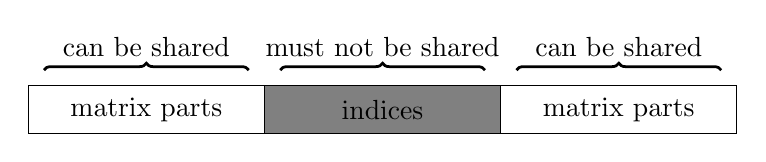
\begin{tikzpicture}[yscale=.6,scale=1]
                        \draw [fill=gray] (3, 2) -- (6, 2) -- (6, 3) -- (3, 3) -- cycle;
                        \draw (0, 2) -- (9, 2) -- (9, 3) -- (0, 3) -- cycle;
                        \draw[dashed] (3, 2) -- (3, 3);
                        \draw[dashed] (6, 2) -- (6, 3);
                        \node(1) at (1.5, 2.5) {matrix parts};
                        \node(2) at (4.5, 2.5) {indices};
                        \node(3) at (7.5, 2.5) {matrix parts};
                        \draw[decorate,line width=1pt,decoration={brace,raise=0.2cm}] (0.2, 3) -- (2.8, 3) node
                        [pos=0.5, yshift=0.5cm] {can be shared};
                        \draw[decorate,line width=1pt,decoration={brace,raise=0.2cm}] (6.2, 3) -- (8.8, 3) node
                        [pos=0.5, yshift=0.5cm] {can be shared};
                        \draw[decorate,line width=1pt,decoration={brace,raise=0.2cm}] (3.2, 3) -- (5.8, 3) node
                        [pos=0.5, yshift=+0.5cm] {must not be shared};
                    \end{tikzpicture}
                \end{minipage}}\vspace{-1em}
            \subfigure[Reusing panel allocation from an iteration to another.\label{fig:panel_reuse}]{\small
                \begin{minipage}[b]{\linewidth}\centering
                    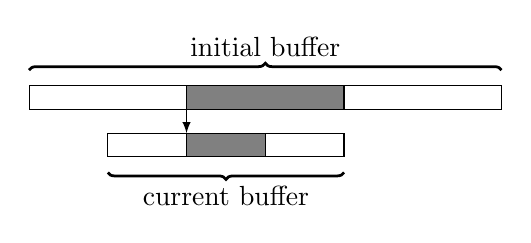
\begin{tikzpicture}[yscale=.6,scale=1]
                        \draw [fill=gray] (2, 1) -- (4, 1) -- (4, 1.5) -- (2, 1.5) --cycle;
                        \draw (0, 1) -- (6, 1) -- (6, 1.5) -- (0, 1.5) -- cycle;
                        \draw[dashed] (2, 1) -- (2, 1.5);
                        \draw[dashed] (4, 1) -- (4, 1.5);

                        \draw [fill=gray] (2, 0) -- (3, 0) -- (3, .5) -- (2, .5) --cycle;
                        \draw (1, 0) -- (4, 0) -- (4, .5) -- (1, .5) -- cycle;
                        \draw[dashed] (2, 0) -- (2, .5);
                        \draw[dashed] (3, 0) -- (3, .5);

                        \draw[-latex] (2, 1) -- (2, .5);
                        \draw[decorate,line width=1pt,decoration={brace,raise=0.2cm}] (0, 1.5) -- (6, 1.5) node
                        [pos=0.5, yshift=0.5cm] {initial buffer};
                        \draw[decorate,line width=1pt,decoration={brace,raise=0.2cm, mirror}] (1, 0) -- (4, 0) node
                        [pos=0.5, yshift=-0.5cm] {current buffer};
                    \end{tikzpicture}
                \end{minipage}%
            }%
            \end{minipage}}%\vspace{-1em}
            \caption{Panel structure and allocation strategy.\label{fig:panel}}\vspace{-1em}
        \end{figure}

        Although using the default \texttt{SHARED\_MALLOC} mechanism works flawlessly for \texttt{A}, a more careful
        strategy needs to be used for the \texttt{panel}, which is an intricate data structure with both \texttt{int}s
        (accounting for matrix indices, error codes, MPI tags, and pivoting information) and \texttt{double}s
        (corresponding to a copy of a sub-matrix of \texttt{A}). To optimize data transfers, HPL flattens this structure
        into a single allocation of \texttt{double}s (see Figure\ref{fig:panel_structure}). Using a fully shared memory
        allocation for the \texttt{panel} therefore leads to index corruption that results in classic invalid memory
        accesses. Since \texttt{int}s and \texttt{double}s are stored in non-contiguous parts of this flat allocation,
        it is therefore essential to have a mechanism that preserves the process-specific content. We have thus
        introduced the \texttt{SMPI\_PARTIAL\_SHARED\_MALLOC} macro that allows us to specify which ranges of the
        allocation should be preserved (\ie are private to each process) and which ones may be corrupted (\ie are shared
        between processes).  For a matrix of order \(40,000\) and \(64\) MPI processes, memory consumption decreases
        with this approach from about \NSI{13.5}{\giga\byte} to less than \NSI{40}{\mega\byte}.

        Another HPL specific optimization is related to the systematic allocation and deallocation of panels in each
        iteration, with the size of the panel strictly decreasing from iteration to iteration. As explained above,
        the partial sharing of panels requires many calls to \texttt{mmap} and introduces an overhead that makes these
        repeated allocations / frees a bottleneck. Since the very first allocation can fit all subsequent panels, we
        modified this allocation mechanism so that SMPI can reuse panels as much as possible from an iteration to an
        other (see Figure\ref{fig:panel_reuse}). Even for a very small matrix of order \(40,000\) and \(64\) MPI
        processes, the simulation time decreases from \NSI{20.5}{\sec} to \NSI{16.5}{\sec}.  The number of page faults
        decreased from \(2\) million to \(0.2\) million, confirming the devastating effect these
        allocations/deallocations would have at scale.

        The next three optimizations are not specific to HPL.  We leveraged the information on which memory area is
        private, shared or partially shared to improve the overall performance.  By making SMPI internally aware of the
        memory's visibility, it can now avoid calling \texttt{memcopy} when large messages containing shared segments
        are sent from one MPI rank to another.  For fully private or partially shared segments, SMPI identifies and
        copies only those parts that are process-dependent (private) into the corresponding buffers on the receiver
        side.  HPL simulation times and memory consumption were considerably improved in our experiments because the
        \texttt{panel} is the most frequently transferred data structure but only a small part of it is actually
        private.

        As explained above, SMPI maps MPI processes to threads of a single process, effectively folding them into the
        same address space.  Consequently, global variables in the MPI application are shared between threads unless
        these variables are \emph{privatized} and the simulated MPI ranks thus isolated from each other. Several
        technical solutions are possible to handle this issue\cite{smpi}. The default strategy in SMPI consists in
        making a copy of the \texttt{data} segment (containing all global variables) per MPI rank at startup and, when
        context switching to another rank, to remap the \texttt{data} segment via \texttt{mmap} to the private copy of
        that rank.  SMPI also implements another mechanism relying on the \texttt{dlopen} function that allows to load
        several times the \texttt{data} segment in memory and to avoid costly calls to \texttt{mmap} (and subsequent
        cache flush) when context switching. For a matrix of order \Num{80000} and \(32\) MPI processes, the number of
        minor page faults drops from \Num{4412047} (with \texttt{mmap}) to \Num{6880} (with \texttt{dlopen}), which
        results in a reduction of system time from \NSI{10.64}{\sec} (out of \NSI{51.47}{\sec}) to \NSI{2.12}{\sec}.

        Finally, for larger matrix orders (\ie \(N\) larger than a few hundred thousands), the performance of the
        simulation quickly deteriorates as the memory consumption rises rapidly. Indeed, folding the memory reduces the
        \emph{physical} memory usage. The \emph{virtual} memory, on the other hand, is still allocated for every process
        since the allocation calls are still executed.  Without a reduction of allocated virtual addresses, the page
        table rapidly becomes too large for a single node. Thankfully, the x86-64 architecture supports several page
        sizes, such as the \emph{huge pages} in Linux. Typically, these pages are around \NSI{2}{\mebi\byte} (instead of
        \NSI{4}{\kibi\byte}), which reduces drastically the page table size. For example, for a matrix of order
        \(N=4,000,000\), it shrinks from \NSI{250}{\giga\byte} to \NSI{0.488}{\giga\byte}.

    \subsection{Scalability Evaluation}
        \begin{figure}[t]
            \centering
            
\includegraphics[width=\linewidth,page=2]{./img/prediction/emulating/scalability_plot_size.pdf}
            \caption{Time complexity and memory consumption are linear in the number of processes but remain mildly
            quadratic with matrix rank.}
            \label{fig:hpl_scalability}
        \end{figure}

        The main goal of the previous optimizations is to reduce the complexity from \(\Theta(N^3) +
        \Theta(N^2\cdot{}P\cdot{}Q)\) to something more reasonable.  The \(\Theta(N^3)\) was removed by skipping most
        computations.  Ideally, since there are \(N/NB\) iterations (steps), the complexity of simulating one step
        should be decreased to something independent of \(N\). SimGrid's fluid models, used to simulate communications,
        do not depend on \(N\). Therefore, the time to simulate a step of HPL should mostly depend on \(P\) and \(Q\).
        Yet, some memory operations on the panel that are related to pivoting are intertwined in HPL with collective
        communications, meaning that it is impossible to get rid of the \(\landauO(N)\) complexity without modifying HPL more
        profoundly.

        To evaluate the efficiency of our proposal, we conduct a first evaluation on a non-existing but Stampede
        resembling platform comprising 4,096 nodes interconnected through a fat-tree topology.
        We run simulations with \Num{512}, \Num{1024}, \Num{2048} or \Num{4096} MPI ranks and with matrices of orders
        \Num{5e5}, \Num{1e6}, \Num{2e6} or \Num{4e6}. All other HPL parameters are similar to the ones of the original
        Stampede scenario.  The impact of the matrix order on total makespan and memory is illustrated in
        Figure\ref{fig:hpl_scalability}.  With all previously described optimizations enabled, the longest simulation
        took close to \(47\) hours and consumed \NSI{16}{\giga\byte} of memory whereas the shortest one took \(20\)
        minutes and \NSI{282}{\mega\byte} of memory.

\section{Modeling HPL kernels and communications}%
\label{sec:prediction:modeling}

    As explained in Section\ref{sec:prediction:emulation}, HPL spends most of its computation time in a dozen specific
    functions for which a performance model has to be designed. Most compute kernels have several parameters from which
    a very simple model can generally easily be identified (\eg proportional to the product of the parameters) but
    refinements including the individual contribution of each parameter as well as the spatial and temporal variability
    of the operation are also possible. Likewise, communications between two nodes are mostly linear in message size but
    the actual performance can wildly vary depending on the range of the message size as MPI switches from one
    protocol to another whenever needed. In this section we first introduce some notations to describe the complexity of
    the models we have investigated. We then briefly compare the prediction of these models with individual measurements
    of both computations and communications to illustrate the importance of the model complexity.

    \subsection{Modeling notations}%

        We denote as \(T\) the duration of an operation with parameters \(M\), \(N\), \(K\) (in the case of the
        \texttt{dgemm} operation, these parameters describe the geometry of the input matrices). We first consider the
        three following modeling options:
        \begin{itemize}
            \item Modeling option \model{0}: For simple and stable compute kernels, the duration can be modeled as a
                constant duration independent of the input parameters, \ie \(T \sim \alpha\), where \(\alpha\) is
                estimated through the sample average of the duration of the operation (or simply 0 if the kernel is
                negligible) .
            \item Modeling option \model{1}: A simple combination of the parameters (\eg \(S=M.N.K\)) may be the primary
                factor driving the performance of the operation. Then \(T \sim \alpha.S ~(+ \beta)\) and \(\alpha\) and
                \(\beta\) can be estimated through a classical least-square linear regression.
            \item Modeling option \model{2}: When the behavior of the operation is complex or requires a faithful
                modeling over the full range of input parameters, a full polynomial model is required, \ie \(T \sim
                \alpha.M.N.K + \beta.M.N + \gamma.N.P + \dots \) Again, the \(\alpha,\beta,\gamma,\dots\) can be
                estimated through a classical least-square linear regression.
        \end{itemize}
        There are two situations where more elaborate variations need to be considered:
        \begin{itemize}
            \item Whenever the platform is slightly heterogeneous (spatial variability), the previous models should be
                built for each host individually. This modeling option is denoted \model[H]{}.
            \item The behavior of the operation may be mostly linear but only for specific parameter ranges. This is for
                example the case for networking operations or for computing nodes on Stampede where Intel's Math Kernel
                Library (MKL) uses the Xeon Phi accelerator only when the input is large enough to compensate for the
                data transfer. In such situations, the models considered will be piece-wise linear, \[\text{e.g., }T
                    \sim \begin{cases} \text{if } M<\theta_1 & \alpha_1.M+\beta_1 \\ \text{else if } M<\theta_2 &
                    \alpha_2.M+\beta_2 \\ ... \end{cases},\] where the \(\theta, \alpha, \beta\) should all be
                    estimated. This kind of model is denoted \modelp{}.
        \end{itemize}
        All previous models can be fit with relatively simple linear regressions or maximum likelihood learning methods.
        However, an important hypothesis underlying all these methods is the homoscedasticity, \ie that the variability
        is independent on the parameters.

        The residual (temporal) variability may be an important phenomenon to account for, as "system noise" is known to
        be detrimental to the overall performance of parallel applications like HPL. We thus consider different modeling
        options for this temporal variability:
        \begin{itemize}
            \item Noise option \noise{0} (no noise): This is the simplest option. It consists in injecting the value
                predicted by the model
            \item Noise option \noise{1} (homoscedastic): The simplest probability family to model variability is the
                normal distribution, hence \(T \sim \model{}(M,N,K) + \norm(0,\sigma^2)\), where \(\sigma^2\) is the
                sample variance of the model residuals.
            \item Noise option \noise{2} (heteroscedastic): The conditional variance of the residuals (\ie \(\sigma^2\)
                given \(M,N,K\)) is modeled by a polynomial function of the input parameters.
        \end{itemize}
        Finally, even the sophisticated normal distribution from \noise{2} may be too simple to describe the noise
        observed on real platforms where it may be common for a same parameter set to have a few operations being one
        order of magnitude slower than all the other ones. In this case, a reasonable option consists of modeling noise
        with a mixture of normal distributions whose parameters \(\pi_1 , \dots, \pi_k\) should be estimated. We denote
        this kind of model as \noisep{}. Likewise, the per-host estimations are denoted by \noise[H]{}.

    \subsection{Modeling  the CPU (\ie \texttt{dgemm} function)}

        \begin{figure}[ht]
            \centering
            \subfigure[\texttt{dgemm}
            heterogeneity\label{fig:dgemm_het}]{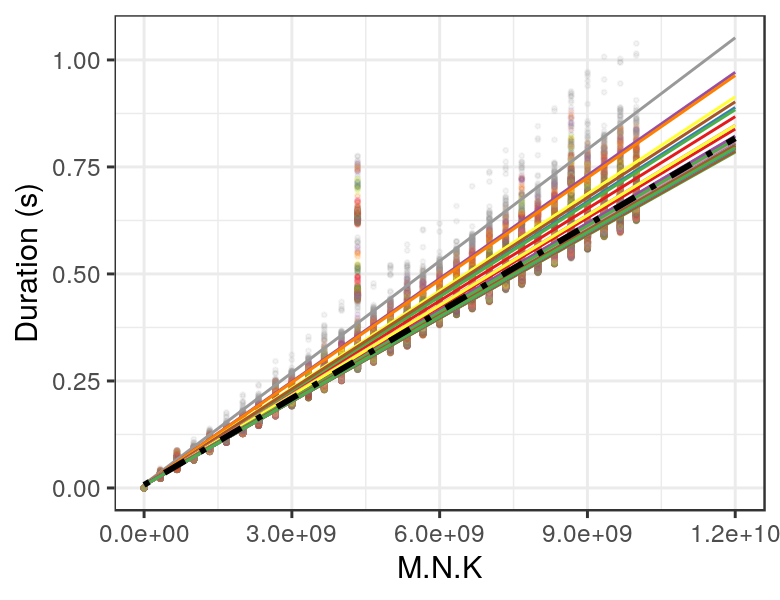
\includegraphics[height=.25\textheight]{img/prediction/modeling/kernels/dgemm_heterogeneity_calib.png}}
            \subfigure[\texttt{dgemm}
            model\label{fig:dgemm_poly}]{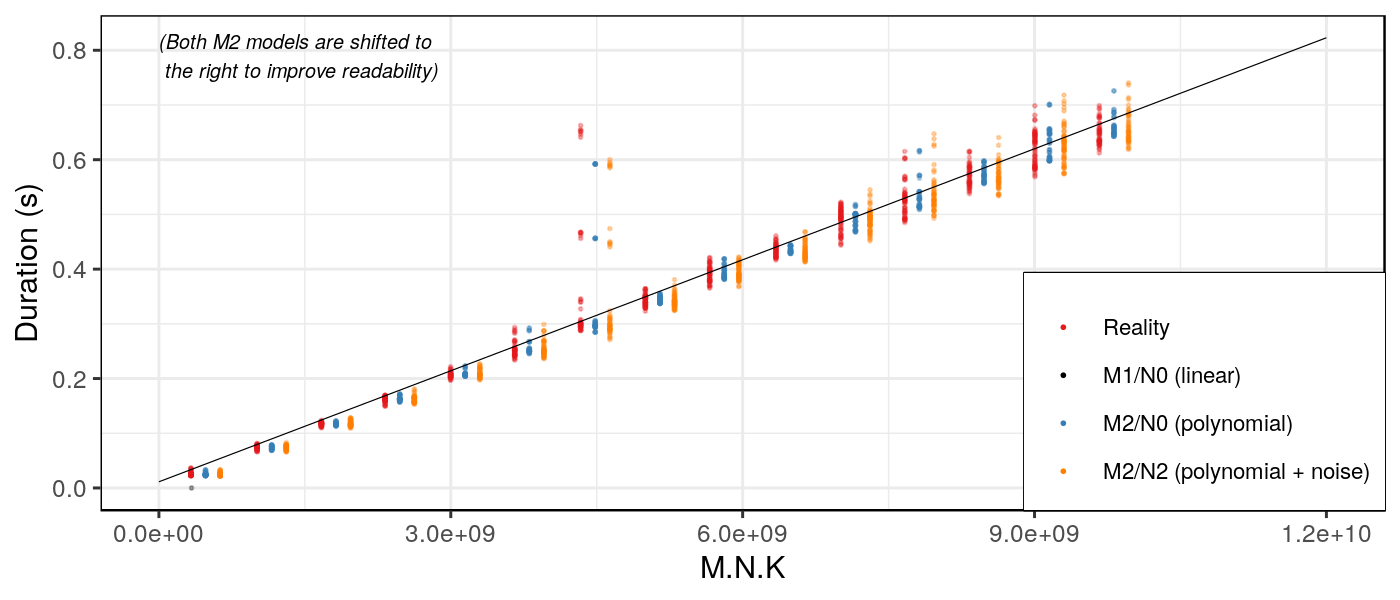
\includegraphics[height=.25\textheight]{img/prediction/modeling/kernels/dgemm_model_calib.png}}
            \caption{Illustrating the realism of modeling for \texttt{dgemm} function}
            \label{fig:blas_var}
        \end{figure}

        HPL spends the most time in the \texttt{dgemm} kernel, it is therefore of extreme importance to model this
        function very faithfully.  We  evaluated the previous modeling alternatives: \model{\{1,2\}}\noise{\{0,1,2\}}
        and \model[H]{\{1,2\}}\noise[H]{\{0,1,2\}}.  The \modelp{} and \noisep{} families were not investigated as
        nothing in our observations called for such complexity on classical multi-core machines.
        Figure\ref{fig:blas_var} illustrates various models and their respective quality for the \texttt{dgemm}
        function. In these figures, the performance of \texttt{dgemm} is evaluated by calling \texttt{dgemm} with
        randomized sizes over all the cores of each node (to reproduce experimental conditions similar to the one of
        HPL). The first observation (Figure\ref{fig:dgemm_het}) is that a few nodes exhibit quite a different behavior
        (each color and each regression line under model \model[H]{1} corresponds to a different cpu, whereas the black
        dotted line corresponds to model \model{1} over all the nodes). These nodes will systematically be slightly
        slower than other nodes and accounting for this spatial heterogeneity is likely to be rather important for HPL.
        Second, we took care of covering a wide variety of combinations for \(M\), \(N\), and \(K\) and it can be
        observed that \(M.N.K\) is not sufficient to describe correctly the performance of \texttt{dgemm}. Indeed, for
        \(M.N.K \approx \num{4.5E9}\) some duration are systematically higher regardless of the node. This happens for
        some particular (e.g., tall and skinny) matrix geometries, which strongly suggests using the full polynomial
        model. Figure\ref{fig:dgemm_poly} depicts the performance (red dots) of a given node as well as the prediction
        using a simple linear model (\model[H]{1}, black line), a full polynomial model (\model[H]{2}, blue dots) and a
        full polynomial model with heteroscedastic noise (\model[H]{2}\noise[H]{2}, orange dots). A close inspection
        reveals that all experimental variability is actually very well explained by both the polynomial model (better
        fit for particular parameter combinations) and some temporal variability.

        \begin{figure}[ht]
            \centering
            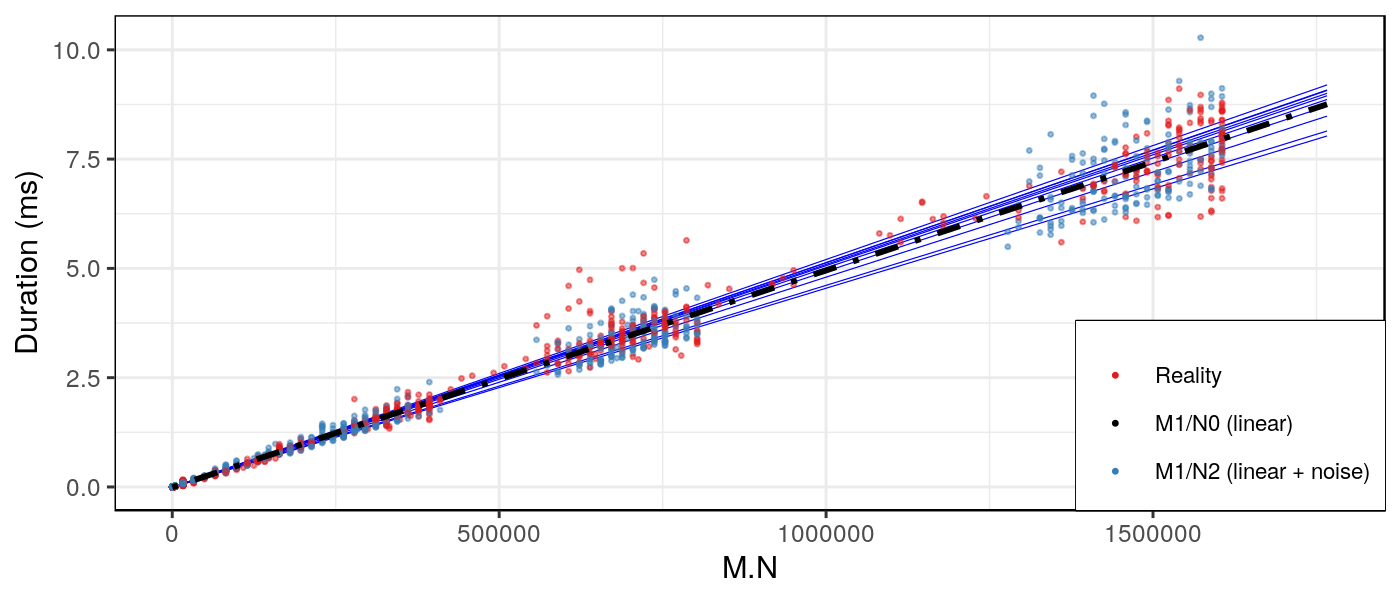
\includegraphics[height=.25\textheight]{img/prediction/modeling/kernels/dlatcpy_model.png}
            \caption{Illustrating the realism of modeling for \texttt{HPL\_dlatcpy} function}
            \label{fig:HPL_var}
        \end{figure}

        Four other BLAS kernels and a few other very small HPL compute kernels (often related to memory management) are
        deeply intertwined with collective operations to allow HPL to be as efficient as possible. Although the total
        duration of these kernels is extremely small compared to the total execution time, they may perturb collective
        communication by introducing late sends and receives. The behavior of one of these kernels is illustrated in
        Figure\ref{fig:HPL_var}. This kind of data can only be obtained by running HPL for a small input matrix over
        each node individually. Again, for all these kernels a single parameter combination explains most of the
        performance and there is some variability from one node to another (one blue regression line per CPU) but it
        remains quite limited (black dotted line for the platform as a whole), especially since these kernels are very
        short and infrequently called compared to \texttt{dgemm}. Finally, since variability significantly increases
        with the value of the input parameters, a \noise{2} model is clearly required. The blue dots in
        Figure\ref{fig:HPL_var} represent the outcome of a \model{1}\noise{2} model and are hardly distinguishable from
        the real behavior. Similar results can be obtained with this category of model for all other kernels.

    \subsection{Modeling the network}

        Prior to this work, the standard way of accounting for protocol changes in SMPI was to estimate breakpoints
        visually and to conduct a linear regression for each range. The expected duration was then used directly in the
        simulation with no particular effort with respect to the temporal variability (\modelp{1}\noise{0}). Yet, as
        illustrated in Figure\ref{fig:nw_var}, the variability of high speed networks is quite particular. We therefore
        diligently estimated all the parameters of \modelp{1}\noisep{1}, where each message size range is automatically
        estimated with \texttt{pytree}, as well as the 2 to 4 modes of the Gaussian mixture for each range. Such
        temporal variability could explain some (overall bad) performance since they generally get amplified by
        broadcast and pipelined communication patterns.

        \begin{figure}[ht]
            \vspace{-1em}
            \centering 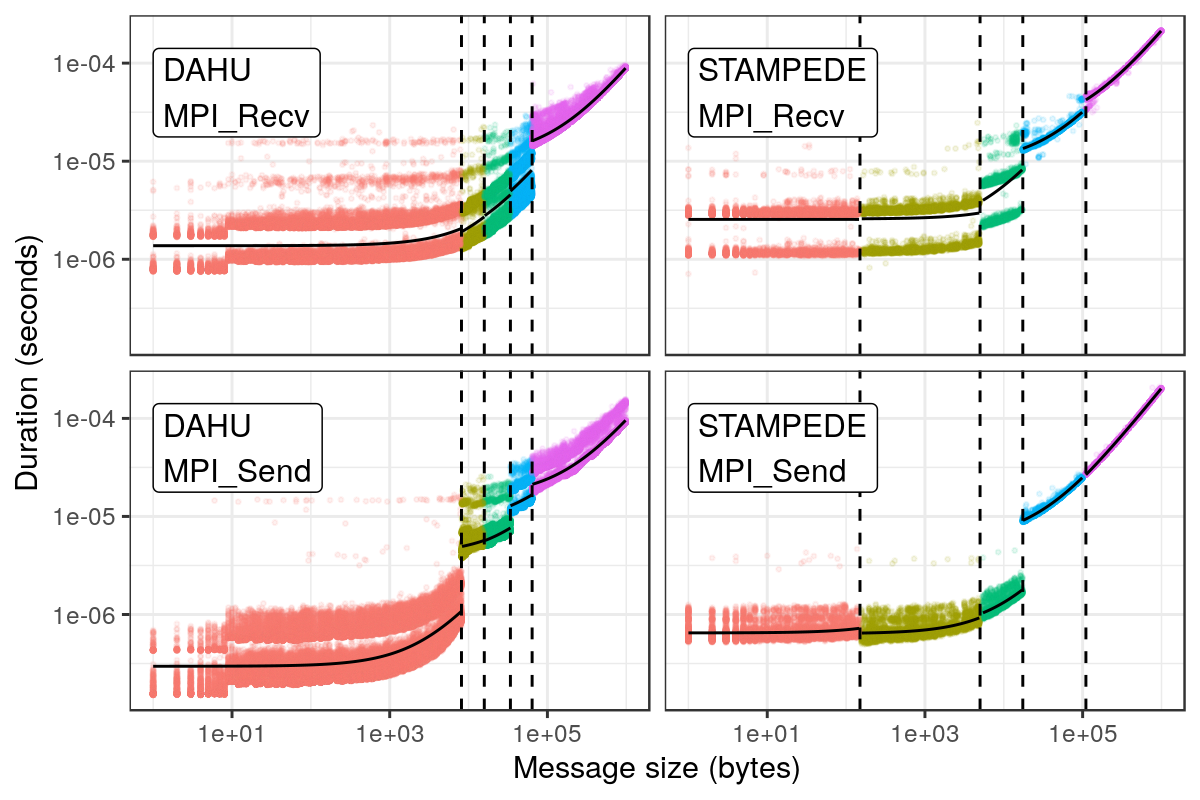
\includegraphics[width=.9\linewidth]{./img/prediction/emulating/mpi_calibration.png}
            \caption{Illustrating piecewise linearity and temporal variability of high-speed communications on two
            systems.}
            \label{fig:nw_var}
        \end{figure}

\section{Validation}%
\label{sec:prediction:validation}

    some text...

\section{Sensibility analysis}%
\label{sec:prediction:sensibility}

    some text...
